\pdfminorversion=4
\documentclass[aps,prl,showpacs,twocolumn,superscriptaddress, floatfix, tightenlines, amsmath, amssymb]{revtex4-1}
\usepackage[pdftex]{graphicx} %[dvips]
\usepackage{natbib}
\usepackage{booktabs}
\usepackage{xcolor}
\usepackage{url}
\usepackage{amsmath}
\usepackage{float}
\usepackage{gensymb}
\usepackage{asypictureB}
\usepackage[utf8]{inputenc}
\usepackage{mathtools}
\usepackage{tikz}
\usetikzlibrary{patterns}
\usepackage[colorlinks=true, citecolor=blue, linkcolor=blue, urlcolor=blue]{hyperref}
\hypersetup{bookmarksnumbered}
\usepackage[bottom]{footmisc}
\usepackage{mwe}
\usepackage{subfig}


\setcounter{tocdepth}{5}
\setcounter{secnumdepth}{5}


\begin{document}

\colorlet{crystal}{violet!75}

\def\zangle{-20}
\def\xangle{20}

\title{An Elementary Introduction to Quantum Cryptography}
\author{Abhiram Cherukupalli}
\date{\today}


\begin{abstract}

Quantum cryptography is one of the most researched fields of Information Theory. New theoretical cryptographic protocols are constantly being developed and realised experimentally. Fundamentally these cryptographic protocols are rendered secure by the laws of quantum mechanics. In this review, we introduce the concepts of quantum mechanics, the idea of measurement collapse, the uncertainty principle and some insightful solutions of the Schr\"{o}dinger Equation. Then, we discuss the EPR paradox, Bell's Theorem leading up to Entanglement and Quantum Cryptography. Next, we examine the Standard Classifications of cryptographic Protocols, the no-cloning theorem, basic protocols like the BB-84 protocol and other similar protocols like bit commitment and entanglement based protocols. Finally, we review their experimental realisations and a few protocols beyond standard key distribution.
\end{abstract}

\maketitle
\tableofcontents
\newpage



\section{Quantum Mechanics Background:}

\subsection{The Wave Function:}


In classical mechanics we can predict the position $x(t)$ and momentum $p(x,t)$ of a particle as a function of time(t) when given the initial conditions and the forces acting on the particle \cite{Griffiths2004Introduction}. However, in quantum mechanics that is not the case. Rather we attempt to find the wave function  $\psi(x,t)$ of the particle.

To calculate this wave function we need to solve the Schr\"{o}dinger equation:
\begin{equation}
i\hbar \frac{\partial \Psi}{\partial t} = -\frac{\hbar^2}{2m}
\frac{\partial^2 \Psi}{\partial x^2} + V \Psi
\label{eq:1}
\end{equation}

This seemingly arbitrary function has an important physical significance, given by Born's statistical interpretation: $\int_a^b |\Psi(x,t)|^2 dx$ signifies the probability of finding a particle between \textit{a} and \textit{b} at a time \textit{t} given its wave function


This means that quantum mechanics is indeterminate, that is, you cannot predict the outcome of any experiment, but you can gain statistical information about all the possible outcomes. However, we can say with certainty that the particle has to be somewhere  in space and time. Therefore, we can normalise the wave function (provided it is square integrable).

\begin{equation}
\int\limits_{-\infty}^\infty |\Psi(x,t)|^2 dx = 1
\label{eq:2}
\end{equation}

This is useful for determining the magnitude of the complex multiplicative factor $A$ (note that we cannot determine the phase of $A$ by normalisation), as if $\psi\left(\mathbit{x},\mathbit{t}\right)$ is a solution to (1), so is $A\cdot{\psi}\left(\mathbit{x},\mathbit{t}\right)$. 


%\begin{multline*}
 % \small \displaystyle f:[a,b]\to \mathbb %{C} {\text{ square integrable on %}}[a,b]\quad \iff \quad\\
  %\int _{a}^{b}|f(x)|^{2}\,\mathrm {d} %x<\infty 
%\label{eq:4}  
%\end{multline*}
\begin{equation}
\begin{split}
\displaystyle f:[a,b]\to \mathbb {C} {\text{ square integrable on }}[a,b]\quad \\
\iff \quad
\int _{a}^{b}|f(x)|^{2},\mathrm {d} x<\infty
\end{split}
\label{eq:3}
\end{equation}

An important consequence of the Schrödinger equation is that if a wave function is normalized at any time, the normalization remains preserved  \cite{Griffiths2004Introduction}.  If the normalization hadn't been preserved, then all wave functions would become non-normalizable (not physical states) and the whole theory would collapse as the Born's interpretation would be deemed incompatible with the Schr\"{o}dinger's equation.


\subsection{What happens when you make a measurement?}

Let us assume an arbitrary wave function of a particle (Figure 1), with probabilities of being at different points.


%ADD MORE

\begin{figure}[H]
\centering
     \includegraphics[width=7.5cm,height=7.5cm,keepaspectratio]{Images/Before2.png}
      \caption{An arbitrary wave function with different probabilities of finding the particle at different points}
       \label{fig:Wavefn}
\end{figure}

\begin{figure}[H]
\centering
     \includegraphics[width=7.5cm,height=7.5cm,keepaspectratio]{Images/After2.png}
      \caption{The collapse of the wave function into a delta function when the particle was found at B }
       \label{fig:collapse}
\end{figure}

The figure in \ref{fig:collapse} represents the Dirac delta function

\begin{equation}
    \delta (x)={\begin{cases}+\infty ,&x=0\\0,&x\neq 0\end{cases}}
    \label{eq:4}\\
    \ \text{Where:} \int _{-\infty }^{\infty }\delta (x)\,dx=1.
\end{equation}



After the measurement, the wave function instantly spreads out, while obeying the Schr\"{o}dinger equation but with different initial conditions, so the wave function gets modified.

Now, the question arises, when we measured the particle to be at B at some time $t_0$ where is B \textit{just before} the measurement?

There are three different positions scientists take on this question:
\begin{enumerate}
\item The realist position: The realist believes that the particle was at C and quantum mechanics could not predict it, making it an ”incomplete theory” that needs a hidden variable along with the wave function for it to be rendered complete. They believed that nothing is indeterminate, and that indeterminacy is just a reflection of our ignorance. 
\item The orthodox position: The particle was not anywhere. You only know where the particle is when you make a measurement, otherwise, its position is indeterminate, and it can be anywhere. We compel the particle to attain a definite position by measuring it. 
\item The agnostic position: The agonist believes that the in-determinacy problem is indeterminable. Because you must make a measurement to know the state of a system, you cannot know the state of a system between measurements. 
\end{enumerate}
Interestingly Albert Einstein was a realist, as he believed quantum mechanics defied causality.

All these positions were popular among scientists until the Bell's theorem was postulated (Sec I.G).\\


This "indeterminacy" of Quantum mechanics leads to a fundamental quantum mechanical principle.

\subsection{Heisenberg Uncertainty Principle:}

There is a famous example to explain the Uncertainty Principle: suppose you have a rope which is tied to a wall on one end and is held by you on the other end. The rope is the "medium" in which the wave travels in.
Now if you periodically move the string up and down and generate a wave (Figure \ref{fig:Wavelength}). We can find the wavelength of this wave, but if you ask me the position of the wave, it would not be defined as the wave is "everywhere" so there is no clearly defined position unlike the wavelength.

\begin{figure}[H]
\centering
     \includegraphics[width=0.5\textwidth]{Images/Heisenberg 1.png}
      \caption{Wave having a well-defined wavelength but an unclear position}
       \label{fig:Wavelength}
\end{figure}

Now what if I produce a wave with a jerk, it is possible to find the position of the wave as the wave is not periodic, so we cannot determine its wavelength.

\begin{figure}[H]
\centering
     \includegraphics[width=0.5\textwidth]{Images/Heisenberg 2.png}
      \caption{Wave having a well-defined position but an unclear Wavelength}
       \label{fig:Position}
\end{figure}

There seems to be a \textit{trade-off} between the precision of wavelength and position: The more precise a wave's position the less precise its wavelength and vice versa.\\

We can relate the wavelength $\lambda$ of the particles wave-function \textbf{$\psi$} with the particle's momentum operator $\hat{p}$ ($\hat{p}\ \Psi(x,t)=\frac{h}{i}\frac{\delta}{\delta x}\Psi(x,t)$) using the de-Broglie's formula:

\begin{equation}
p=\frac{h}{\lambda}=\frac{2\pi\hbar}{\lambda}
\label{eq:5}
\end{equation}

So, if the wavelength of the particle is less precise, its momentum is also less precise and its position is more precise.
Mathematically the Heisenberg Principle is given by:
\begin{equation}
\Delta x * \Delta p  \geq \frac{\hbar}{2}
\label{eq:6}
\end{equation}

Here, $\Delta x$ and $\Delta p$ represent the uncertainties in position ad momentum respectively. The Heisenberg Principle represents a trade-off between precision of the measurement of position and momentum.

\subsection{Time-invariant Schr\"{o}dinger's Equation}

When we come to solve the Schr\"{o}dinger's Equation, for simplicity we try to find separable solutions for the wave function. Separable wave functions are simple products:

\begin{equation}
\Psi(x,t) = \mathit{\psi}(x)*f(t) 
\label{eq:7}
\end{equation}
 
Where $\mathit{\psi}$ does not depend on t and f does not depend on x. Such separable solutions are important, because as we will see soon when we combine separable solutions we can obtain a general solution. If we assume the wave function is separable then we can simplify the Schr\"{o}dinger equation to obtain: 

\begin{equation}
-\frac{\hbar^2}{2m} \frac{d^2 \psi}{dx^2} + V\psi = E\psi \\
\label{eq:8}
\end{equation}

\eqref{eq:8} is known as the time invariant Schr\"{o}dinger Equation (V is assumed to be independent of time). 

The wave function that is obtained from this Equation is:

\begin{equation}
\Psi(x,t) = {\psi}(x) * e^{\frac{-iEt}{\hbar}}
\label{eq:9}
\end{equation}

Notation: $\psi$ is only a function of x whereas $\Psi$ is a function of both x and t.

The separable wave function in \eqref{eq:9} is important because of 3 reasons:

\begin{enumerate}


 

\item  \textbf{They have a definite total energy}: 
The Hamiltonian in classical mechanics is the sum of kinetic and potential energies of the system:
 
\begin{equation}
H(x, p) =\frac{p^2}{2m}+V(x)
\label{eq:10}
\end{equation}

By substituting p as $\frac{h}{i}\frac{\delta}{\delta x}$ in \eqref{eq:10} we get the Hamiltonian operator to be:

\begin{equation}
\hat{H} =-\frac{\hbar^2}{2m}*\frac{\delta^2}{\delta x^2}+V(x)
\label{eq:11}
\end{equation}

So the Schr\"{o}dinger equation can be written as:
\begin{equation}
    \hat{H}\psi=E\psi
    \label{eq:12}
\end{equation}

Hence for any separable solution, the value of the total energy must always return the value E \cite{Griffiths2004Introduction}.

\item The general solution to the Schr\"{o}dinger Equation \eqref{eq:1} is a \textbf{linear combination of separable solutions}.
\begin{equation}
\Psi_1(x,t) = {\psi}(x) * e^{\frac{-iE_1t}{\hbar}}, \Psi_2(x,t) = {\psi}(x) * e^{\frac{-iE_2t}{\hbar}},...
\end{equation} Each wave function has its own corresponding energy, so there is a different $\Psi$ for each energy level.

\begin{equation}
    \Psi(x,t)= \sum_{n=1}^{\infty} c_n\psi_n(x,t)  e^{\frac{-iE_nt}{\hbar}} = 1
\end{equation}

It happens to be that every general solution to the Schr\"{o}dinger equation can be expressed as a linear combination of separable wave-functions, all we need to do is adjust the constant $c_n$.
\item  \textbf{It renders a stationary problem}:
Though the wave function in \eqref{eq:9} has a time-dependent factor, the probability function doesn't.
This is because $|\Psi(x,t)|^2=\Psi^{*}(x,t)\times \Psi(x,t)$, hence the time dependent factor cancels out
\begin{subequations}
\begin{equation}
\small |\Psi(x,t)|^2 = \Psi^*\times \Psi = \psi(x)e^{\frac{-iEt}{\hbar}} \times \psi^* (x)e^{\frac{+iEt}{\hbar}} \\ = |\psi(x)|^2
\label{eq:10}
\end{equation}
\end{subequations}

Note that we could cancel out E in \eqref{eq:10} because for normalizable solutions E must be real \cite{Griffiths2004Introduction}. 

\end{enumerate}

\subsection{Particular solutions of the time-independent Schr\"{o}dinger equation}
To better understand the intricacies of the laws of quantum mechanics let us take a look at a few particular solutions of the Schr\"{o}dinger equation.
\subsubsection{The Free Particle}

This a very simple, yet insightful, solution of the Schr\"{o}dinger equation. Here, V(x)=0 everywhere and as a consequence of Schr\"{o}dinger equation $E>V_{min}$ for all normalizable solutions. This implies that the free particle, due to the absence of any boundary conditions, can have any positive energy.

Putting this into \eqref{eq:8} we get

\begin{equation}
-\frac{\hbar^2}{2m} \frac{d^2 \psi}{dx^2} = E\psi
\label{eq:16}
\end{equation}

The resulting differential equation's solution can be written as:

\begin{equation}
\psi(x) = A e^{ikx}+ Be^{-ikx}
\label{eq:17}
\end{equation}

With $k=\frac{\sqrt{2mE}}{h}$ (from \eqref{eq:16})

\begin{equation}
    \small
    \Psi(x, t) = \psi(x)*e^\frac{-iEt}{\hbar}=A e^{ik(x-\frac{\hbar k}{2m}t)}+ Be^{-ik(x+\frac{\hbar k}{2m}t)}
\end{equation}

But we know that whenever a continuous function f(x,t) obeys the wave equation \eqref{eq:19}, it represents a wave

\begin{equation}
    \frac{{\partial ^2 f(x,t)}}{{\partial x^2 }} = \frac{1}{{c^2 }}\frac{{\partial ^2 f(x,t)}}{{\partial t^2 }}
    \label{eq:19}
\end{equation}
Where c is the speed of the wave.

Then if at time $t=0$, the wave was represented by f(x) then at time $t_0$ the wave is represented by $f(x-vt_0)$ as the x-axis has translated to the right at rate of v m/s.

\begin{figure}[H]
\centering
     \includegraphics[width=0.5\textwidth]{Images/Movewavefinal.png}
      \caption{A wave which is given by f(x) at t=0 is given by $f(x-vt_0)$ at t=$t_0$}
       \label{fig:Position}
\end{figure}


In this case the velocity is $\frac{\hbar k}{2m} = \sqrt\frac{E}{2m}$ as $k=\frac{\sqrt{2mE}}{h}$

But if this was a classical particle its energy would be $E= \frac{1}{2}mv^2$ $\Rightarrow$ $v=\sqrt\frac{2E}{m}$

How is this possible for the classical speed to be double that of the quantum mechanical speed? 
To understand this let us imagine a wave packet in which there is a sinusoidal wave contained. The classical particle velocity represents the velocity of the whole envelope (group velocity) whereas the wave velocity (phase velocity) represents the velocity of the waves contained in it.

\begin{figure}[H]
\centering
     \includegraphics[width=0.5\textwidth]{Images/Wave Packet.png}
      \caption{A wave packet. The envelope moves at the group velocity $v_g$. Whereas the waves inside it move at the phase velocity $v_p$}
       \label{fig:Position}
\end{figure}

A real life example of the distinction between $v_g$ and $v_p$ is given by waves of water, though the water itself travels in a single direction, say left to right, the particles of water inside it move in elliptical paths, as their motion is a superposition of transverse and longitudinal motions, and the eccentricity depends on the depth of the water. 
\begin{figure}[H]
\centering
     \includegraphics[width=0.5\textwidth]{Images/Motion-of-a-particle-in-an-ocean-wave-A-At-deep-water-The-orbital-motion-of-fluid.png}
      \caption{Motion of a Particle of Water inside a water wave as a superposition of both longitudinal and transverse motions, the particles end up taking elliptical paths (Wikimedia Commons)}
       \label{fig:wave}
\end{figure}


If we look closely at the free particle's wave function we notice that it is non-normalizable, implying that it doesn't represent a physical state. Though that's the case, the free-particle example is still one of great importance as it gives us useful insight into quantum mechanics.

\subsubsection{The Infinite square well}

Another important case is when $V(x)$ behaves kind of like a delta function, suppose $V(x)=0$ from $0\leq x \leq a$ but V(x)=$\infty$ elsewhere. The particle behaves as a free particle from $0\leq x \leq a$ until it reaches the ends which it cannot cross so it "bounces" back.

\begin{figure}[H]
    \centering
    \includegraphics[scale=0.6]{Images/Infinite square well.png}
    \caption{The infinite square well}
    \label{fig:infinite square well}
\end{figure}

If we write \eqref{eq:17} in trigonometric form we get:

\begin{equation}
    \psi(x)=A\sin{kx}+B\cos{kx}
\end{equation}

$\psi(0)=\psi(a)=0$ (as $\psi$ when $x < 0$ and $> a$ is 0 and $\psi$ is continuous). So B =0
\begin{equation}
    \psi(a)=A\sin{ka}=0;
    k = \frac{\pm n\pi}{a}
\end{equation}

\begin{equation}
E_n=\frac{\hbar^2k^2}{2m}= \frac{\hbar^2n^2\pi^2}{2ma^2} (\text{from \eqref{eq:16}})
\end{equation}
Also,
\begin{equation}
 \psi_n(x)= \sqrt\frac{2}{a}sin(\frac{n\pi}{a}); (A= \sqrt\frac{2}{a} \text{ from normalisation})
\label{eq:23}
\end{equation}


This means that a particle in the infinite square well can only have a set of allowed values of energy. n=1 has the lowest energy and is called as the ground states all other values of $n>1$ are called as excited states ($n=0$ is rejected as you would not be able to normalise the wave function). This example gives us a peek into the core of quantum mechanics: quantization.

Important note: All the wave functions $\psi_n(x)$ are mutually orthogonal:
\begin{equation}
   \int(\psi_m(x)^* \psi_n(x))=0 \; ( m \neq n)
   \label{eq:24}
\end{equation}

If any two wave-functions obey \eqref{eq:23} we say they are orthogonal.

\subsubsection{The Harmonic Oscillator}

To further our understanding of quantization let us consider another example of typical harmonic oscillations of a block of mass m attached to a spring of spring constant k. 

\begin{equation}
    F=-kx=ma=m\frac{d^2x}{dt^2}
\end{equation}
\begin{equation}
    x= Asin(wt)+Bcos(wt); \; w= \sqrt\frac{k}{m}
\end{equation}

\begin{equation}
V(x) = \frac{1}{2}kx^2
\end{equation}

We can approximate any oscillation to be a simple harmonic motion (a type of periodic motion where the restoring force is proprtional to displacement and acts towards the mean position), via a parabolic approximation provided the amplitude is small.

\begin{figure}[H]
\centering
     \includegraphics[width=0.5\textwidth]{Images/Parabolic Approximation.png}
      \caption{In the small region around a local minimum we can always assume the graph is parabolic (via the Taylor series expansion of V(x)) }
       \label{fig:Position}
\end{figure}
\begin{equation}
    -\frac{\hbar^2}{2m} \frac{d^2 \psi}{dx^2} + \frac{1}{2}m\omega^2x^2 = E\psi
\end{equation}

If we simplify this expression we can use the fact that: $a^2+b^2=(a+ib)(a-ib)$
\begin{equation}
\frac{1}{\sqrt{2m}}(\frac{\hbar}{i}\frac{d}{dx} + im\omega x)*\frac{1}{\sqrt{2m}}(\frac{\hbar}{i}\frac{d}{dx} - im\omega x)= E\psi
\end{equation}

Let us denote the first term as $a_+=\frac{1}{\sqrt{2m}}(\frac{\hbar}{i}\frac{d}{dx} + im\omega x)$ and $a_-=\frac{1}{\sqrt{2m}}(\frac{\hbar}{i}\frac{d}{dx} - im\omega x)$

These are called the ladder operators because they have a special property:
If $\psi$ obeys the Schr\"{o}dinger's equation, with an energy E, then $a_+\psi$ obeys the Schr\"{o}dinger's equation with an energy $E+\hbar\omega$ and same applies for $a_-$. Now we can see why they are called the ladder operators, $a_+$ allows us to climb the quantized ladder of energy whereas $a_-$ makes us descend it.

\begin{figure}[H]
\centering
     \includegraphics[width=7.5cm,height=7.5cm,keepaspectratio]{Images/Ladder Operators.png}
      \caption{The ladder operators and the quantized ladder }
       \label{fig:Position}
\end{figure}


This is another good example of the Schr\"{o}dinger which kind of gives an intuitive feel for quantization. Also, it is important to note that quantum mechanics predicts that particles can cross a infinite barrier, quantum tunneling, which has been proven to be the case and is now used in scanning tunneling microscopy \cite{binnig_rohrer_1987}.



\subsection{The EPR paradox:}
Coming back to our discussion of what happens when we take a measurement, Einstein, Podolsky and Rosen believed in the realist interpretation. These three came up with the infamous EPR paradox.




Assume we have a neutral pi meson (of zero spin) which decays to produces a electron-positron pair, $\pi^0\to e^- + e^+ $. Since spin angular momentum should be conserved, the spin of the electron and positron must be opposite in sign. Therefore, if the spin of the electron is measured as spin up $\uparrow$, the spin of the positron as spin down $\downarrow$ is automatically measured. Quantum mechanics cannot tell you what the spin would be deterministically. All it tells you that no matter how far apart they are their measured spins must be of opposite parity. This implies that as soon as one of the particle’s spin is measured, the wave function of the other particle collapses instantaneously. Einstein and other realists felt such “spooky action at a distance" to be impossible, because if the mutual wave function collapse was instantaneous, then the travel speed of the causal influence between them appears to be faster than  light. A Paradox!

\begin{figure}[H]
    \centering
    \includegraphics[scale=0.6]{Images/EPR.png}
    \caption{Two Particles very far away always have the opposite spin, as if there is some sort of spring attached to them}
    \label{fig:my_label}
\end{figure}

The realists believe that the electron always had spin up since the time it was made and, quantum mechanics being incomplete, was not able to predict the spin as it needed some hidden variable to be complete. They did not believe quantum mechanics to be wrong, they believed it was incomplete. 

\subsection{Bell's Theorem:}
Different hidden variable theories were put forward forward in the following decades, but none were considered plausible. Considerable theoretical work was put into finding a hidden variable theory, but without success until J.S. Bell came along, who proved that any hidden variable theory is incompatible with quantum mechanics \cite{PhysicsPhysiqueFizika.1.195}.
The idea is as follows: We orient the detectors in a non-parallel direction, allowing them to rotate freely. Let $P(a,b)$ denote the average of the product of the spins measured by the detectors oriented along unit vectors a and b, 

\begin{figure}[H]
    \centering
    \includegraphics[scale=0.5]{Images/Bell Configuration.png}
    \caption{The Bell configuration non-parallel detectors}
    \label{fig:my_label}
\end{figure}
If $b=a$, then we get back the original EPR orientation so $P(a,a)=1$, similarly $P(a,-a)=-1$. Quantum mechanics predicts that for any configuration $(a,b)$ 
\begin{equation}
    P(a,b)=-a*b
\end{equation}
If there is a hidden variable needed to describe the complete state of both the particles, then some new functions $A(a,\lambda)$ and $B(b,\lambda)$ give the results of the electron and positron measurement successfully (Here we assume that the electron measurement is independent of orientation of b). 
We can see that $A(\vec{a},\lambda)=-B(\vec{a},\lambda)$. Also:
\begin{equation}
    \small P(\vec{a},\vec{b})=\int \rho(\lambda)A(\vec{a},\lambda)B(\vec{b},\lambda)d\lambda=-\int \rho(\lambda A(\vec{a},\lambda)A(\vec{b},\lambda)d\lambda
    \label{eq:31}
\end{equation}

If $\vec{c}$ is another unit vector, on simplifying \eqref{eq:31} we arrive at:

\begin{equation}
\mid P(\vec{a},\vec{b})-P(\vec{a},\vec{c})\mid \leq 1+P(\vec{b},\vec{c})
\label{Bell}
\end{equation}

This can be proven to be inconsistent with quantum mechanics by taking all three vectors in the same plane with \textbf{b} and \textbf{c} making angle 45° and 90° with \textbf{a} respectively. Clearly the inequality in \eqref{Bell} will not hold, implying that there can be no hidden variable theory that can save us from the non-locality of quantum mechanics.

The Bell's inequality was tested in 1970 by Aspect, Grangier and Roger \cite{PhysRevLett.47.460} and the results were in agreement with quantum mechanical prediction and was incompatible with the Bell's inequality. This shocked the physics research world as this proves nature being fundamentally non-local. 
But why is non-locality so disturbing? How can the influence between the electron and positron travel faster than light? 

To explain this, we have to make an important distinction: A causal influence cannot travel faster than the speed of light, but other influences, such as instantaneous wave collapse, could. The latter influences carry no energy; hence, they are by no circumstance bound to be traveling slower than light. This is proven by the no-communication theorem, which states that during the measurement of one of the particles, it is not possible for one observer to communicate information to another observer, thereby preserving causality. 

\section{Quantum Entanglement}

States such as the EPR pair, where there is an inherent dependency of one particles measurement on the other, are called entangled states. 
Any composite state of two quantum systems A and B can be represented as: $H_A \otimes H_B$ where $H_A$ and $H_B$ are their respective Hilbert Spaces having base states $\{|{a_{i}}\rangle \otimes |{b_{j}}\rangle \},$ and$\otimes$ represents the tensor product. So, $$\displaystyle |\psi \rangle =\sum _{i,j}c_{i,j}(|a_{i}\rangle \otimes |b_{j}\rangle )=\sum _{i,j}c_{i,j}|a_{i}b_{j}\rangle $$

If $|\psi \rangle \in H_{1}\otimes H_{2}$ can be written as $|\psi \rangle =|\psi _{1}\rangle \otimes |\psi _{2}\rangle $ the state is said to be separable, otherwise it is entangled.

For example, the EPR configuration can be represented as:
$$\tfrac{1}{\sqrt{2}} \left ( |0\rangle_A \otimes |1\rangle_B - |1\rangle_A \otimes |0\rangle_B \right )$$

It is impossible to separate this wave function into $|\psi \rangle =|\psi _{A}\rangle \otimes |\psi _{B}\rangle$, thus making this configuration entangled. If Observer A measures 0, the state of the system becomes $ |0\rangle_A |1\rangle_B$ and vice versa.

\section{The Idea of Quantum Cryptography}

"No measurement can be made without perturbing the system." 
This unusual property of quantum mechanics underlies the core concept involved in secure communication channels. If, for example, two people, Alice and Bob, want to communicate with each other quantum information (e.g., photons carrying the information). Eve, an eavesdropper, cannot obtain any information without perturbing the system, thus revealing her presence. Alice and Bob can simply check whether someone is eavesdropping by comparing the data that is passed through the public channel. This would be of no use, though, as they will get to know of eavesdropping after the data transfer takes place. However, when this idea is complemented with a key, it can ensure privacy before any data transfer. A key is a random sequence of bits (qubits), which is sent through the channel. If the key is unperturbed, it means the data channel is secure, so the parties can start sending information encoded in the keys \cite{RevModPhys_QuantumCryptography_2002, RevModPhys_quantumkeydistribution_2020}.
\section{Cryptography:}
Cryptography is the science of constructing protocols that prevent eavesdroppers from reading private encrypted messages. An algorithm can be used to achieve this, with the help of a key to encrypt the message. For it to be considered secure, it should be impossible to unlock a cryptosystem without its key. Modern cryptosystems can be broadly divided into two categories. 
\begin{itemize}
  \item \textbf{Asymmetrical cryptosystems:} Also known as public-key cryptosystems, Alice and Bob use different keys. Bob prepares a public key using a secret private key and Alice uses this public key to encrypt a message which can \textbf{only} be decrypted by Bob's private key. 
  A classical version of this protocol is prime factorisation. Given the prime factors of a large number, it is easy to compute the number but it becomes much harder in the other direction (Computing $127\cdot 71\cdot 7$ is easy but given $63119$ it is much harder to find the prime factors). That is, a type of an one way function. Fortunately, the backward process can be made easier if one of the factors is known, in this case the key. However, prime factorisation isn't  "proven" to be secure.
  \begin{figure}[H]
      \centering
      \includegraphics[scale =0.5]{Images/Asymettrical.png}
      \caption{An Asymmetrical cryptosystem where different keys are used encrypt and decrypt}
      \label{fig:Sy}
  \end{figure}
  
  \item \textbf{Symmetrical cryptosystems:} Both Alice and Bob use the same private key to encrypt and decrypt the message. Let us assume, Alice adds a key (k) to the message (m) in a binary system ($s=m \otimes k$) now Bob can simply subtract $k$ from Alice's message and decrypt it. This system is provably secure because $s$ is as random as $m$ and hence it doesn't contain any information so it is provably secure. However, notable disadvantages exist with this cryptosystem: Alice and Bob must posses the same private key (which must be longer than the message it self). This key must be pre-shared in a secure manner and also should necessarily be used only once (like an one time password). This is because, if the same key is used twice Eve can gain some information about the messages by just adding the public messages ($s_A\otimes s_B = m_A\otimes k\otimes m_B \otimes k = m_1\otimes m_B $, using commutation). Interestingly, asymmetrical cryptosystems are often used to send the private sessions key used in symmetrical cryptosystems.
  
\end{itemize}
  \begin{figure}[H]
      \centering
      \includegraphics[scale =0.5]{Images/Symettrical.png}
      \caption{An Symmetrical cryptosystem where the same key is used encrypt and decrypt}
      \label{fig:Asy}
  \end{figure}



If these cryptographic algorithms were broken by advances in mathematics, Quantum Cryptography would be the only solution.


\section{Shannon Information Theory}

Information can be thought of in terms of randomness, that is, entropy or probability. If a certain event is likely to occur, you gain lesser information from it; higher the probability of occurrence lesser is the information transferred. This entropy is represented mathematically by using Shannon Entropy or Information entropy (H):
\begin{equation}
    {\displaystyle H=-\sum _{j}p_{j}\log _{2}(p_{j})}
    \label{Shannon_1}
\end{equation}

where $p_j$ is probability of occurrence of $j^{th}$ value. Shannon, continued this discussion, in 1984 by proving that no matter how noisy a channel is, it is possible to communicate data, almost error free, up to a \textbf{maximum number} known as the channel capacity which only depends on the statistics of the channel \cite{shannon}.

\begin{equation}
    C=B \text{$^2\log (1+\frac{S}{N}$)}
\end{equation}

where C is the channel capacity (maximum bit rate), B is the bandwidth of the Channel, $\frac{S}{N}$ is the signal-to-noise ratio where S is the average signal power received and N is the average power of the noise. Similarly, we can think of this quantum mechanically, where Eve gains information from a quantum tunnel between Alice and bob at the cost of introducing noise into the system which lowers the bit rate. It is a constant tug of war between perturbation and information.

\begin{figure}[H]
\centering
     \includegraphics[width=8cm,height=8cm,keepaspectratio]{Images/Perturbation Information.png}
      \caption{The tug of war between perturbation and information }
       \label{fig:Tug Of War}
\end{figure}

\section{The No-Cloning theorem:}

Suppose Eve intercepts the message between Alice and Bob, she could just measure the quantum state and then resend a duplicate of it without perturbing the system, staying "undetected".

Conveniently as a consequence of quantum mechanics it can be proven that "no arbitrary quantum state can be perfectly cloned". This is the no-cloning theorem. An intuitive proof for this statement is that if we could make perfect copies, then the person could make as many identical copies as he wanted and measure every parameter with arbitrary precision, thereby breaking the uncertainty principle.

However, remember that the no-cloning theorem only prevents against making perfect copies, but you can make as many "imperfect" copies as you want.

Its important to note than non-orthogonal states can never be perfectly cloned so whatever Eve does should bring in some errors.


\begin{figure}[H]
    \centering
    \includegraphics[scale = 0.3]{Images/Noclone1.png}
    \caption{Depiction of an ideal copying machine which clones the states $|0\rangle$ and $|1\rangle$ perfectly}
    \label{fig:my_label}
\end{figure}
\begin{figure}[H]
    \centering
    \includegraphics[scale = 0.25]{Images/Noclone2.png}
    \caption{If such an ideal cloning machine did exist then it would give the wrong answer for the superposition state of $|0\rangle + |1\rangle$\cite{nocloningintuitive}}
    \label{fig:my_label}
\end{figure}   


\section{The BB-84 Protocol:}

This protocol, aptly called the BB84 protocol, was proposed by Charles H. Bennett and Gilles Brassard in 1984 at the IEEE conference in India \cite{Bennett_2014}. In this protocol Alice encodes the bit in a polarization state of a photon in one of two non-orthogonal bases either rectilinear or diagonal. The binary $0$ state is defined as 0° polarization in the rectilinear state or a 45° polarization in the diagonal state. Similarly, a Binary 1 state is defined as 90° polarization in the rectilinear state or a 135° polarization in the diagonal state.

\begin{figure}[H]
\centering
     \includegraphics[width=5cm,height=5cm,keepaspectratio]{Images/polarized.jpeg}
      \caption{polarized states in the BB84 Protocol }
      
\end{figure}
\begin{figure}[H]
\centering
     \includegraphics[width=5cm,height=5cm,keepaspectratio]{Images/BB 84 basis.png}
      \caption{The Bases of BB 84 protocol }
      \centering
       \label{fig:BB84.}
\end{figure}
Initially, Alice sends a key to Bob over a quantum channel. First, she chooses a random string of bits (for the binary states) and a basis for each bit to get a polarized state. Alice then sends her qubits to Bob, who measures the photons using a random non-orthogonal basis. If Bob chooses the same basis as Alice then he would get the same polarization (if no one eavesdropped on the photon). If, however, Bob chooses a different basis the qubits he reads would be random. Next, Bob discloses the bases he chose to Alice over a public channel (but, importantly, he does not disclose his result). Alice reports which bases are correlated and they discard the other bits where the bases are not correlated. If Eve does not eavesdrop on the channel both Alice and Bob would have the same perfectly correlated key called the sifted key. However, the crucial step, is that both Alice and Bob agree upon a random subset of the bits, and they compare them. If there is no measurement error or noise in the channel, the bits will be perfectly correlated and if they are no, it reveals the presence of Eve, who modified the photon by measuring it. If there was a measurement error, then error correction protocol can be used (Sec X.). Due to the Quantum No-cloning Theorem, Eve cannot replicate the photon she measures as she doesn't know with certainty the quantum state of the photon. 

However, how safe really is this protocol? To answer, let us assume Eve intercepts the photon (an imperfect copy) and re-sends it to Bob (the intercept-resend strategy). Eve has to guess the random base and she has a $50\%$ chance of guessing it right. A total of $25\%$ of Bob's bases will be uncorrelated which gives Eve a \textbf{maximum} of $75\%$ probability of not being detected. If the string of bits is long enough this probability will tend to 0 (as it depends on ${(\frac{3}{4})}^n$) \cite{Pirandola_2020}.



\section{The One time pad:}

Classically, a One time pad can be achieved if Alice and Bob have an arbitrarily long pre-shared secret key which is used to encrypt and decrypt the messages. In theory, Alice could measure her classical system with arbitrarily high precision and then use the one-time pad to securely communicate this information to Bob, who can then, in principle, reconstruct (a copy of) the classical system. This however will not work in a Quantum Cryptographic Algorithm.

Let us say Alice wants to send a copy of a quantum system to Bob, she cannot do that as that violate the no-cloning theorem. However, they could sharea quantum key and a classical channel. Alice could "teleport" her quantum state to Bob without gaining any information about the quantum state, while Bob would end up with a state isomorphic with the original state (but he doesn't learn anything about the quantum state). This was aptly called "quantum teleportation" \cite{Bennet93}. 

This is the only provably secure QC, you can show that if the quantum channel used to the share the key was secure, so is the one time pad \cite{bellovin_2011, peng_cui_song_2021}.
\section{Other similar protocols:}

\subsection{Quantum Bit commitment and Coin-tossing:}
\subsubsection{Bit commitment:}
Continuing with our two communicating parties, let us suppose that Alice chooses a bit (0 or 1), which she commits to, and wants to show Bob the evidence that she, indeed, has a bit in mind and cannot alter it.  However, with this evidence, Bob should not be able to figure out the bit Alice chose. In case Alice changes her bit after commitment, it is considered as cheating, which a bit commitment protocol should protect against.

As it surprising turns out, there can never exist any bit-commitment protocol which is secure! This can be proved rigorously \cite{Chiribella_2013}, but I would like to focus more on the implications of the impossibility of a bit-commitment protocol, it means that we could never trust Alice! She could cheat all she wants without Bob finding out. 
\subsubsection{Coin Flipping:}
Similar to the idea of bit-commitment is that of coin flipping. Assume Alice and Bob are far away from each other and playing a game. The idea of the game is that one of Alice and Bob, say Alice, flips a coin, and the other, Bob, guesses the face of the coin. If the guess is correct, then Bob wins. Otherwise, Alice wins. However, in a classical coin tossing game, we could never know if Alice cheated. Of course, with the use of a trusted third party who flips the coin this problem is solved, but what if we could make a protocol that solely relied on the laws of quantum mechanics to ensure no cheating in this coin-flipping game without the help of any third party. If a secure bit-commitment protocol was available, then making this coin-flipping scheme would be trivial (But, importantly not the other way around). It just so happens that as long as Alice and Bob do not share any entangled state, any quantum flipping scheme would be impossible. Another really fascinating outcome of quantum mechanics! It shows that Alice can really cheat if she wanted without Bob finding anything out \cite{Coin_Flip}.

For a while it was believed that these classical protocols have "provably unbreakable" quantum counterparts, but quantum bit commitment and ideal coin tossing was also proven to not be secure \cite{qbcimpossible}.



\subsection{Entanglement-Based Protocols using the Bell's theorem:}

\subsubsection{Eckert E91 protocol:}

In this protocol a quantum channel sends two entangled particles (preferably polarized photons) one each for Alice and Bob. They choose on a random basis and they correct their raw keys, as in the BB84 protocol to obtain the sifted keys. If there was no eavesdropping, Bob's key would be the perfect complement of Alice's key. Here is the interesting part: to know whether Eve was peeking into the quantum channel, all they need to do is measure the photons where they used two different bases, now they measure the photons in a third predetermined base and then compare their results. If their results obeyed the Bell's inequality (which does not hold for entangled particles), it reveals the presence of Eve as the photons are no longer entangled\cite{PhysRevLett.67.661}.
\begin{figure}[H]
    \centering
    \includegraphics[scale =.2]{Images/Entangled E91.png}
    \caption{The Eckert entanglement protocol}
    \label{e91}
\end{figure}

\subsubsection{BBM92 Protocol and Other Variants:}

Bennet and Brassard in 1992 made a variation of the E91 protocol which does not require the Bell's test. Similar to the E91 protocol there is an entangled photon source, Alice and Bob make measurements on a random basis, and they publicly announced their bases. Therefore, when they are correlated the spin must be opposite. If it isn't, it reveals the presence of Eve. Furthermore, Bennet and Brassard proved that any variant of the BB84 protocol could be adapted to use an entangled photon source without the use of the Bell test  \cite{bb92}. Enzer, in 2002, proposed another entanglement-based protocol, which is an entangled version of the Six-State Protocol \cite{bennett_brassard_crepeau_maurer_1915}.

\begin{figure}[H]
\centering


\tikzset{every picture/.style={line width=0.75pt}} %set default line width to 0.75pt        

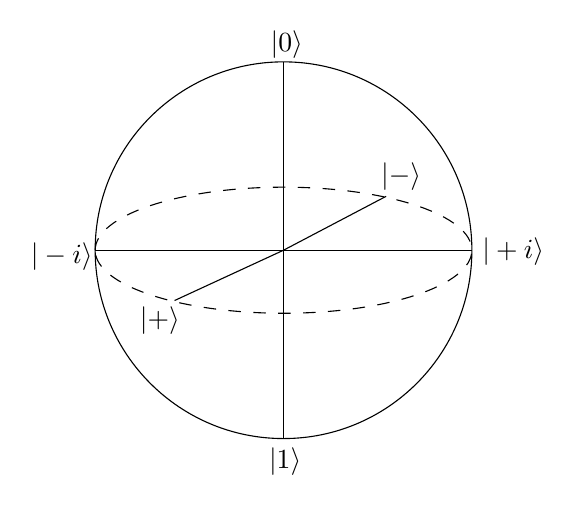
\begin{tikzpicture}[x=0.75pt,y=0.75pt,yscale=-1,xscale=1, scale =.75]
%uncomment if require: \path (0,300); %set diagram left start at 0, and has height of 300

%Shape: Circle [id:dp4522432438865791] 
\draw   (200,146) .. controls (200,79.17) and (254.17,25) .. (321,25) .. controls (387.83,25) and (442,79.17) .. (442,146) .. controls (442,212.83) and (387.83,267) .. (321,267) .. controls (254.17,267) and (200,212.83) .. (200,146) -- cycle ;
%Straight Lines [id:da9578485023820269] 
\draw    (321,25) -- (321,267) ;
%Straight Lines [id:da7136589561932805] 
\draw    (200,146) -- (442,146) ;
%Straight Lines [id:da6079127393917905] 
\draw    (321,146) -- (251,178.33) ;
%Straight Lines [id:da7572958846518187] 
\draw    (386.87,111.4) -- (321,146) ;
%Shape: Ellipse [id:dp7021570994359627] 
\draw  [dash pattern={on 4.5pt off 4.5pt}] (200,146) .. controls (200,123.63) and (254.17,105.5) .. (321,105.5) .. controls (387.83,105.5) and (442,123.63) .. (442,146) .. controls (442,168.37) and (387.83,186.5) .. (321,186.5) .. controls (254.17,186.5) and (200,168.37) .. (200,146) -- cycle ;

% Text Node
\draw (227,180.4) node [anchor=north west][inner sep=0.75pt]    {$|+\rangle $};
% Text Node
\draw (382,88.4) node [anchor=north west][inner sep=0.75pt]    {$|-\rangle $};
% Text Node
\draw (447,136.4) node [anchor=north west][inner sep=0.75pt]    {$|+i\rangle $};
% Text Node
\draw (157,139.4) node [anchor=north west][inner sep=0.75pt]    {$|-i\rangle $};
% Text Node
\draw (311,3.4) node [anchor=north west][inner sep=0.75pt]    {$|0\rangle $};
% Text Node
\draw (310,271.4) node [anchor=north west][inner sep=0.75pt]    {$|1\rangle $};


\end{tikzpicture}

\caption{The Six State Protocol} \label{fig:M1}
\end{figure}



\section{Eavesdroppers, Their strategies and How to Counter Them:}

If their bases are correlated, Alice and Bob should, in theory, have identical sifted keys. However, in reality that is not the case as there are many errors that are introduced, which eavesdroppers capitalise on. To counter them we need to apply some information protocols:

\begin{enumerate}
    \item \textbf{Error Correction:} The error rate, called the quantum bit error rate, QBER (to avoid confusion with the classical Bit error rate BER) is usually of the order of a few percent. This error rate would be reduced down to the order of $10^{-9} \%$  using classical algorithms.
    \item \textbf{Privacy Amplification:} After error correction, both Alice and Bob have the same sifted keys. However, Eve might still have information; this is where privacy amplification comes in. It reduces the information Eve has to almost zero. We assume that Alice, Bob and Eve respectively have the variables $\alpha, \beta, \epsilon$ and their entire probability distribution is given by P($\alpha, \beta, \epsilon$). Both Alice and Bob know what P($\alpha, \beta$) is, and from \eqref{eq:35} we can get a lower bound on $S(\alpha, \beta|| \epsilon)$ in terms of the difference between Alice and Bob's mutual information $I(\alpha, \beta)$ and Eve's mutual information \cite{RevModPhys_QuantumCryptography_2002}.
    \begin{equation}
        S(\alpha, \beta|| \epsilon) \geq \text{max\{$I(\alpha, \beta)-I(\alpha,\epsilon),I(\alpha, \beta)-I(\alpha,\epsilon)$\}}
        \label{eq:35}
    \end{equation}

    To establish a secret key using this idea, Alice and Bob compare a random subset of their sifted keys and estimate the QBER. If \eqref{eq:35} is not satisfied ,they stop the protocol, and if it is satisfied they continue on with error correction protocols. In other words, as Alice and Bob share an identical key, they can transform their key into a new shortened key in such a way that Eve cannot gain information unless she also has an identical key. Therefore, even if Eve has substantial information on the key, it would be of no use after privacy amplification. 
\end{enumerate}
\flushle
The aim of eavesdropping analysis is to find "ultimate proofs" (security that works against all types of eavesdropping attacks) for cryptosystems. Eavesdropping attacks that Eve carries out are broadly classified into two categories:
\begin{enumerate}
    \item Individual attacks: Here, Eve attaches independent probes to each photon individually, and measures each probe, one at a time. It is also known as an Incoherent Attack.
    \item Joint attacks: In the most general case of a joint attack, Eve can measure multiple probes at once coherently; hence, they are also called coherent attacks. A commonly used subset of a joint attack is the collective attack, which assumes that each photon is probed only once but many probes can be measured at once.
\end{enumerate}

Individual attacks can be translated into a classical problem using the idea of privacy amplification of imposing constraints on the joint probability distribution using the laws of quantum mechanics.

\subsection{The Intercept resend strategy:}

Assuming we use the BB84 protocol, we know that there is a $25\%$ QBER and Eve gains $0.5$ bits of information for each qubit measured. From Shannon Information theory, we know that the amount of information Eve gains is the amount of entropy decrease.
\begin{equation}
    I(\alpha, \epsilon) = -\Delta H
    \label{eq:36}
\end{equation}
where $ I(\alpha, \epsilon)$ denotes how much information Eve $\epsilon$ has on Alice and H is the Shannon entropy. We can simplify \eqref{eq:36} using \eqref{Shannon_1} and the fact that $H_{initial}$ is 1 as Alice's bit is uniform. We find, as expected, that Eve gains 1/2 a bit for each qubit measured.
\begin{equation}
    h(p) = p\log_2(p)+(1-p)\log_2(1-p)
    \label{eq:intercept}
\end{equation}
In addition, the probability of Eve guessing the correct bit is $0.75$ (as expected). However, if Eve measures the bit in an intermediate basis, the Breidbart Basis.
\begin{figure}[H]
\centering
     \includegraphics[scale=0.3]{Images/briedbart2.png}
      \caption{The Breidbart Basis}
       \label{fig:Briendart}
\end{figure}
Then the probability that she gets the bit correct is $cos^2\frac{\pi}{8}=0.85$ and curiously by using \eqref{eq:intercept}, we find that Eve only gains 0.4 bits per qubit but has a higher probability of getting it right, this is because in the Breidbart basis in half of the cases the information is deterministic, but in the regular BB84 protocol the information is always probabilistic. 

\subsection{"Ultimate" security proofs for any noisy channel:}

In an ideal channel with no noise, it is easy to prove that quantum cryptography (QC) is secure. However, it is interesting to note that this proof can be extended to any noisy channel provided the equipment is perfect. Obviously, QC is only secure up to a threshold of QBER which is what we need to find. The proof provided in \cite{RevModPhys_QuantumCryptography_2002} uses two theorems: 
\\
\textbf{Theorem 1}. For a given joint distribution P($\alpha, \beta, \epsilon$), Alice and Bob can form a shared secret key if and only if $I(\alpha, \beta) \geq I(\alpha, \epsilon)$ or $I(\alpha, \beta) \geq I(\beta, \epsilon)$. In other words, this means that Bob must have more knowledge on Alice's bits than Eve does. This can be understood visually in the figure below.


\begin{figure}[H]
    \centering
    \includegraphics[scale = 0.6]{Images/Privacy amplification.png}
    \caption{A feel for Theorem 1. The initial situation is given in 1. After Error Correction Bob's information becomes 1. After Privacy Amplification, Eve's information becomes 0. As Bob disregarded all the random bits so he loses information. And finally, scrapping this random bits gives us a secret key.}
    \label{fig:my_label}
\end{figure}

\textbf{Theorem 2}. If Eve performs a
measurement giving her some information $I(\alpha, \epsilon)$, then, because of the perturbation, there is a limit on the amount of information Bob can gain.

If n is the number of qubits,which Bob receives, that are in the same basis then Theorem 2 implies that:
\begin{equation}
    I(\alpha, \epsilon) + I(\alpha, \beta) \leq n
\end{equation}

Essentially information per qubit both Bob and Eve gained when combined should be $\leq$ 1. Combined with \eqref{eq:intercept} we obtain:
\begin{equation}
    QBER \leq 11\%
    \label{eq:39}
\end{equation}

Therefore, whenever \eqref{eq:39} is obeyed an ultimate security protocol can be developed. Note that this proof is valid only when the key is much longer than the number of qubits Eve intercepts.

\section{Two way quantum communication protocols:}

Two-way quantum protocols have a distinct advantage over unidirectional protocols in that they are deterministic. Generally, in a two-way protocol, Bob prepares quantum states and sends them to Alice via the quantum channel, who encodes the states and re-sends it back to Bob, who performs a measurement. There are two common two-way protocols: The LM-05 protocol and the ping pong protocol.

\subsection{LM-05 protocol:}
Here Bob sends of qubit in one the forms $|0\rangle$, $|1\rangle$, $|+\rangle$, $|-\rangle$. Alice does one of two things to this qubit, she either uses this qubit as a control to test  with a probability of $c$ (control mode) or uses it to encode information (encoding mode),  with a probability of $1-c$. The way Alice tests for noise is similar to the BB84 protocol, wherein she measures the qubit on a random basis. In the original protocol, Alice now sends the qubit back with the exact same wavelength, amplitude, time gap, or else Eve could determine Alice's chosen mode. However, this is not feasible in real life. Instead, Alice encodes this bit into information and re-sends it to Bob, who decodes it using the same base he sent the qubit in. As we can observe, this is a deterministic protocol as Bob know Alice's bases without a need for base-reconciliation which would be non-deterministic. In addition, for the two-way tunnel protocol to work, a direct test on at least one direction of the tunnel is necessary. Therefore, a two-way quantum tunnel protocol is susceptible to attacks such as the Trojan horse attack (Sec XII.C). without the control mode \cite{lucamarini_deterministic_2005, lucamarini_secure_2005}.
\begin{figure}[H]
    \centering
\includegraphics[scale=0.3]{Images/LM05.png}
    \caption{The LM-05 Protocol: Bob Prepares a Qubit and sends it to Alice who uses the qubit as a control or to encode information. She sends the encoded bit to Bob who decodes it.}
    \label{LM05}
\end{figure}

\subsection{Ping Pong Protocol:}

In the ping-pong protocol, an entangled orthogonal 
state is used in the following form:

\begin{equation*}
\begin{aligned}
    |\phi^{\pm}\rangle=\frac{1}{\sqrt{2}}(|0\rangle|0\rangle\pm|1\rangle|1\rangle) \newline
     |\psi^{\pm}\rangle=\frac{1}{\sqrt{2}}(|0\rangle|1\rangle \pm|1\rangle|0\rangle) 
     \end{aligned}
\end{equation*}

As you can see they are just the EPR states. What Bob does is that he makes two, qubits one being the home qubit and the other being the travel qubit. Bob sends this travel qubit $|\psi^+\rangle$ to Alice who randomly chooses whether to do a message mode or control mode. Let us asuume that Alice chooses the message mode and encodes the qubit she received from Bob using an encoding operation $\sigma_\alpha^b$ where b is either 0 or1. If $b=0$ then the qubit $|\psi^+\rangle$ will be transformed into $|\psi^-\rangle$. However, if $b=1$ it will be left untouched. Alice sends this encoded bit to Bob who performs a Bell measurement to get the wave function to be one of $|\psi^+\rangle$, $|\psi^-\rangle$ hence revealing the value of b \cite{5515357}.

If instead Alice chooses the control mode, she measures the qu-bit in basis {$|0\rangle$, $|1\rangle$} and then reveals the result publicly to Bob, now Bob also makes a measurement in the basis {$|0\rangle$, $|1\rangle$} and announces his result. If their results do not differ it indicates the presence of Eve and the protocol is aborted.


\section{Real life examples:}

\subsection{Photon Number Splitting (PNS) Attacks}
The entanglement protocols are difficult to work with in real life, as modern-day equipment cannot reliably produce and measure singular photons. In real life, a laser produces a number of coherent photons. Eve can exploit this by splitting off a small number of photons for each qubit and lets the rest of the photons pass on to Bob, leaving no trace. This attack is called the photon number splitting or PNS attack \cite{PhysRevLett.85.1330}.
\begin{figure}[H]
    \centering


\tikzset{every picture/.style={line width=0.75pt}} %set default line width to 0.75pt        

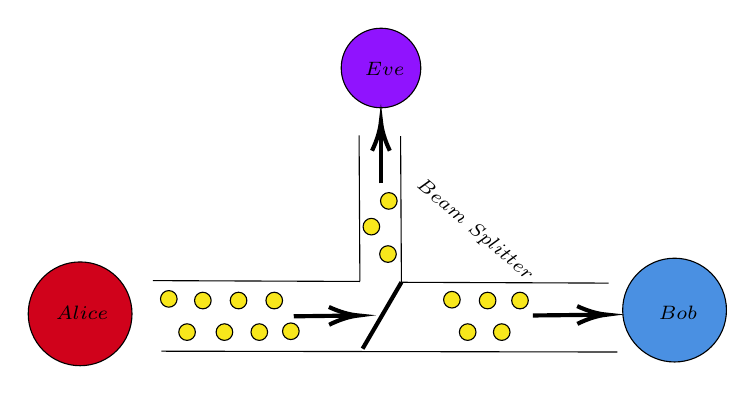
\begin{tikzpicture}[x=0.75pt,y=0.75pt,yscale=-1,xscale=1]
%uncomment if require: \path (0,300); %set diagram left start at 0, and has height of 300

%Shape: Circle [id:dp11707720901437169] 
\draw  [fill={rgb, 255:red, 208; green, 2; blue, 27 }  ,fill opacity=1 ] (100.4,166.2) .. controls (100.4,152.39) and (111.59,141.2) .. (125.4,141.2) .. controls (139.21,141.2) and (150.4,152.39) .. (150.4,166.2) .. controls (150.4,180.01) and (139.21,191.2) .. (125.4,191.2) .. controls (111.59,191.2) and (100.4,180.01) .. (100.4,166.2) -- cycle ;
%Straight Lines [id:da6192032972458446] 
\draw    (160.4,150.2) -- (260.2,150.6) ;
%Straight Lines [id:da263180448091209] 
\draw    (164.6,184.2) -- (384.2,184.6) ;
%Straight Lines [id:da5071614891362606] 
\draw    (260.2,150.6) -- (259.8,80.2) ;
%Straight Lines [id:da4240422536526136] 
\draw    (280.2,151) -- (279.8,80.6) ;
%Straight Lines [id:da08917818350636275] 
\draw    (280.2,151) -- (380,151.4) ;
%Shape: Circle [id:dp6853698329061144] 
\draw  [fill={rgb, 255:red, 74; green, 144; blue, 226 }  ,fill opacity=1 ] (386.8,164.4) .. controls (386.8,150.59) and (397.99,139.4) .. (411.8,139.4) .. controls (425.61,139.4) and (436.8,150.59) .. (436.8,164.4) .. controls (436.8,178.21) and (425.61,189.4) .. (411.8,189.4) .. controls (397.99,189.4) and (386.8,178.21) .. (386.8,164.4) -- cycle ;
%Shape: Circle [id:dp8208497916913471] 
\draw  [fill={rgb, 255:red, 248; green, 231; blue, 28 }  ,fill opacity=1 ] (164.13,159) .. controls (164.13,156.79) and (165.92,155) .. (168.13,155) .. controls (170.34,155) and (172.13,156.79) .. (172.13,159) .. controls (172.13,161.21) and (170.34,163) .. (168.13,163) .. controls (165.92,163) and (164.13,161.21) .. (164.13,159) -- cycle ;
%Shape: Circle [id:dp020126958969106212] 
\draw  [fill={rgb, 255:red, 248; green, 231; blue, 28 }  ,fill opacity=1 ] (172.93,175) .. controls (172.93,172.79) and (174.72,171) .. (176.93,171) .. controls (179.14,171) and (180.93,172.79) .. (180.93,175) .. controls (180.93,177.21) and (179.14,179) .. (176.93,179) .. controls (174.72,179) and (172.93,177.21) .. (172.93,175) -- cycle ;
%Shape: Circle [id:dp5196149281970122] 
\draw  [fill={rgb, 255:red, 248; green, 231; blue, 28 }  ,fill opacity=1 ] (180.53,159.8) .. controls (180.53,157.59) and (182.32,155.8) .. (184.53,155.8) .. controls (186.74,155.8) and (188.53,157.59) .. (188.53,159.8) .. controls (188.53,162.01) and (186.74,163.8) .. (184.53,163.8) .. controls (182.32,163.8) and (180.53,162.01) .. (180.53,159.8) -- cycle ;
%Shape: Circle [id:dp6728435855245942] 
\draw  [fill={rgb, 255:red, 248; green, 231; blue, 28 }  ,fill opacity=1 ] (190.93,175) .. controls (190.93,172.79) and (192.72,171) .. (194.93,171) .. controls (197.14,171) and (198.93,172.79) .. (198.93,175) .. controls (198.93,177.21) and (197.14,179) .. (194.93,179) .. controls (192.72,179) and (190.93,177.21) .. (190.93,175) -- cycle ;
%Shape: Circle [id:dp6173714661331138] 
\draw  [fill={rgb, 255:red, 248; green, 231; blue, 28 }  ,fill opacity=1 ] (197.73,159.8) .. controls (197.73,157.59) and (199.52,155.8) .. (201.73,155.8) .. controls (203.94,155.8) and (205.73,157.59) .. (205.73,159.8) .. controls (205.73,162.01) and (203.94,163.8) .. (201.73,163.8) .. controls (199.52,163.8) and (197.73,162.01) .. (197.73,159.8) -- cycle ;
%Shape: Circle [id:dp6980445137260738] 
\draw  [fill={rgb, 255:red, 248; green, 231; blue, 28 }  ,fill opacity=1 ] (207.73,175) .. controls (207.73,172.79) and (209.52,171) .. (211.73,171) .. controls (213.94,171) and (215.73,172.79) .. (215.73,175) .. controls (215.73,177.21) and (213.94,179) .. (211.73,179) .. controls (209.52,179) and (207.73,177.21) .. (207.73,175) -- cycle ;
%Shape: Circle [id:dp2359199198275701] 
\draw  [fill={rgb, 255:red, 248; green, 231; blue, 28 }  ,fill opacity=1 ] (261.73,124.2) .. controls (261.73,121.99) and (263.52,120.2) .. (265.73,120.2) .. controls (267.94,120.2) and (269.73,121.99) .. (269.73,124.2) .. controls (269.73,126.41) and (267.94,128.2) .. (265.73,128.2) .. controls (263.52,128.2) and (261.73,126.41) .. (261.73,124.2) -- cycle ;
%Shape: Circle [id:dp1268318025732007] 
\draw  [fill={rgb, 255:red, 248; green, 231; blue, 28 }  ,fill opacity=1 ] (270.13,111.8) .. controls (270.13,109.59) and (271.92,107.8) .. (274.13,107.8) .. controls (276.34,107.8) and (278.13,109.59) .. (278.13,111.8) .. controls (278.13,114.01) and (276.34,115.8) .. (274.13,115.8) .. controls (271.92,115.8) and (270.13,114.01) .. (270.13,111.8) -- cycle ;
%Shape: Circle [id:dp8191443385511872] 
\draw  [fill={rgb, 255:red, 248; green, 231; blue, 28 }  ,fill opacity=1 ] (269.73,137.4) .. controls (269.73,135.19) and (271.52,133.4) .. (273.73,133.4) .. controls (275.94,133.4) and (277.73,135.19) .. (277.73,137.4) .. controls (277.73,139.61) and (275.94,141.4) .. (273.73,141.4) .. controls (271.52,141.4) and (269.73,139.61) .. (269.73,137.4) -- cycle ;
%Shape: Circle [id:dp11758309613480922] 
\draw  [fill={rgb, 255:red, 144; green, 19; blue, 254 }  ,fill opacity=1 ] (251.2,47.77) .. controls (251.2,37.18) and (259.78,28.6) .. (270.37,28.6) .. controls (280.95,28.6) and (289.53,37.18) .. (289.53,47.77) .. controls (289.53,58.35) and (280.95,66.93) .. (270.37,66.93) .. controls (259.78,66.93) and (251.2,58.35) .. (251.2,47.77) -- cycle ;
%Shape: Circle [id:dp613789405137884] 
\draw  [fill={rgb, 255:red, 248; green, 231; blue, 28 }  ,fill opacity=1 ] (300.53,159.4) .. controls (300.53,157.19) and (302.32,155.4) .. (304.53,155.4) .. controls (306.74,155.4) and (308.53,157.19) .. (308.53,159.4) .. controls (308.53,161.61) and (306.74,163.4) .. (304.53,163.4) .. controls (302.32,163.4) and (300.53,161.61) .. (300.53,159.4) -- cycle ;
%Shape: Circle [id:dp4627248515273126] 
\draw  [fill={rgb, 255:red, 248; green, 231; blue, 28 }  ,fill opacity=1 ] (308.13,175) .. controls (308.13,172.79) and (309.92,171) .. (312.13,171) .. controls (314.34,171) and (316.13,172.79) .. (316.13,175) .. controls (316.13,177.21) and (314.34,179) .. (312.13,179) .. controls (309.92,179) and (308.13,177.21) .. (308.13,175) -- cycle ;
%Shape: Circle [id:dp8219418792265456] 
\draw  [fill={rgb, 255:red, 248; green, 231; blue, 28 }  ,fill opacity=1 ] (317.73,159.8) .. controls (317.73,157.59) and (319.52,155.8) .. (321.73,155.8) .. controls (323.94,155.8) and (325.73,157.59) .. (325.73,159.8) .. controls (325.73,162.01) and (323.94,163.8) .. (321.73,163.8) .. controls (319.52,163.8) and (317.73,162.01) .. (317.73,159.8) -- cycle ;
%Shape: Circle [id:dp47532330345974017] 
\draw  [fill={rgb, 255:red, 248; green, 231; blue, 28 }  ,fill opacity=1 ] (324.53,175) .. controls (324.53,172.79) and (326.32,171) .. (328.53,171) .. controls (330.74,171) and (332.53,172.79) .. (332.53,175) .. controls (332.53,177.21) and (330.74,179) .. (328.53,179) .. controls (326.32,179) and (324.53,177.21) .. (324.53,175) -- cycle ;
%Shape: Circle [id:dp033441291589944466] 
\draw  [fill={rgb, 255:red, 248; green, 231; blue, 28 }  ,fill opacity=1 ] (214.93,159.8) .. controls (214.93,157.59) and (216.72,155.8) .. (218.93,155.8) .. controls (221.14,155.8) and (222.93,157.59) .. (222.93,159.8) .. controls (222.93,162.01) and (221.14,163.8) .. (218.93,163.8) .. controls (216.72,163.8) and (214.93,162.01) .. (214.93,159.8) -- cycle ;
%Shape: Circle [id:dp2526467281066127] 
\draw  [fill={rgb, 255:red, 248; green, 231; blue, 28 }  ,fill opacity=1 ] (333.33,159.8) .. controls (333.33,157.59) and (335.12,155.8) .. (337.33,155.8) .. controls (339.54,155.8) and (341.33,157.59) .. (341.33,159.8) .. controls (341.33,162.01) and (339.54,163.8) .. (337.33,163.8) .. controls (335.12,163.8) and (333.33,162.01) .. (333.33,159.8) -- cycle ;
%Straight Lines [id:da17535896882331148] 
\draw [line width=1.5]    (228.33,167.4) -- (256.53,167.04) ;
\draw [shift={(259.53,167)}, rotate = 179.27] [color={rgb, 255:red, 0; green, 0; blue, 0 }  ][line width=1.5]    (14.21,-4.28) .. controls (9.04,-1.82) and (4.3,-0.39) .. (0,0) .. controls (4.3,0.39) and (9.04,1.82) .. (14.21,4.28)   ;
%Straight Lines [id:da3674396766186716] 
\draw [line width=1.5]    (270.33,103.4) -- (270.33,76.4) ;
\draw [shift={(270.33,73.4)}, rotate = 90] [color={rgb, 255:red, 0; green, 0; blue, 0 }  ][line width=1.5]    (14.21,-4.28) .. controls (9.04,-1.82) and (4.3,-0.39) .. (0,0) .. controls (4.3,0.39) and (9.04,1.82) .. (14.21,4.28)   ;
%Shape: Circle [id:dp6367379340465176] 
\draw  [fill={rgb, 255:red, 248; green, 231; blue, 28 }  ,fill opacity=1 ] (222.93,174.6) .. controls (222.93,172.39) and (224.72,170.6) .. (226.93,170.6) .. controls (229.14,170.6) and (230.93,172.39) .. (230.93,174.6) .. controls (230.93,176.81) and (229.14,178.6) .. (226.93,178.6) .. controls (224.72,178.6) and (222.93,176.81) .. (222.93,174.6) -- cycle ;
%Straight Lines [id:da1722030679373796] 
\draw [line width=1.5]    (343.53,167) -- (376.13,166.63) ;
\draw [shift={(379.13,166.6)}, rotate = 179.36] [color={rgb, 255:red, 0; green, 0; blue, 0 }  ][line width=1.5]    (14.21,-4.28) .. controls (9.04,-1.82) and (4.3,-0.39) .. (0,0) .. controls (4.3,0.39) and (9.04,1.82) .. (14.21,4.28)   ;
%Straight Lines [id:da5993348900824433] 
\draw [color={rgb, 255:red, 0; green, 0; blue, 0 }  ,draw opacity=1 ][line width=1.5]    (280.2,151) -- (261.5,183) ;

% Text Node
\draw (112.53,161.2) node [anchor=north west][inner sep=0.75pt]  [font=\scriptsize]  {$Alice$};
% Text Node
\draw (261.33,43.6) node [anchor=north west][inner sep=0.75pt]  [font=\scriptsize]  {$Eve$};
% Text Node
\draw (402.93,161.2) node [anchor=north west][inner sep=0.75pt]  [font=\scriptsize]  {$Bob$};
% Text Node
\draw (291.23,98.22) node [anchor=north west][inner sep=0.75pt]  [font=\scriptsize,rotate=-40.18]  {$Beam\ Splitter$};


\end{tikzpicture}
    \caption{The PNS attack, Eve uses a Beam Splitter to Divert some Photons to her without perturbing Bob's Measurement but gaining a small amount of information.}
    \label{fig:my_label}
\end{figure}

This attack can be countered in two ways: the first is the SARG-04 protocol where Alice does not reveal her bases publicly but reveals a pair of non-orthogonal states in which the bit might be encoded in. If Bob measures on the same basis, he would have measured one of the non-orthogonal states and, if not, they simply discard the bit. Now, all Eve can do is guess, so her Shannon information is significantly lower \cite{PhysRevLett.91.057901}. Unfortunately, the SARG-04 protocol, which was theorized to be the same as the BB-84 protocol, but experimentally it under performs due to errors introduced \cite{Jeong_2014}.\newline

The second method uses decoy pulses where Alice sends the beams of varying intensities, with only one being the signal pulse and all others being decoy pulses. The so called "Decoy State Protocol". With the help of these decoy pulses Alice can detect the presence of Eve as she cannot maintain the bit error rate when multi-photon sources are involved \cite{PhysRevLett.91.057901, PhysRevLett.94.230504, Wang_2005}.\newline
Accounting for more such real-life quantum channel imperfections, Gottesmann's paper \cite{10.5555/2011586.2011587} explains the real life security of BB84-based protocols.


\subsection{Intensity based attacks:}


When Huang tested the decoy state protocol in real life using a source that could regulate the intensity, he found that different intensities in general corresponded to different times at which the pulses were sent \cite{Huang_2018}. This means theoretically, Eve can differentiate between a decoy pulse and the actual signal according to the time of sending. However, Alice can counter this attack by modulating the intensity of the photons after they are sent, and it was found that when an external modulator was used, all photons were simultaneous. However, as recently discovered Eve can heat up Alice's source using high-intensity sources, and this shifts the timings of different intensity pulses, Alice cannot compensate for this time delay unless she finds out that they have been changed \cite{Fei_2018}.

\subsection{Trojan horse and Back-flash attacks:}

Trojan horse attacks are a classical case of QC, which reminds us that the security of QC is not determined just by the laws of Quantum mechanics but it also depends on the technical measures. In this attack, Eve sends a light pulse through a quantum channel, in this case an optical fiber, entering Alice's or Bob's detector, and then Eve analyzes the reflected light. This provides her information about the polarization settings of the apparatus by calculating the phase shift. We cannot however, simply just block the optical fiber as it would not allow for communication between Alice and Bob. To be protected against this attack, Alice should first reduce the time period ($\Delta t_{phase})$ in which a phase shift occurs to the order of nanoseconds, forcing Eve to send the pulse at the same time as Bob. Next, Alice using an attenuator reduces the energy of the pulse from Bob to, let's say 0.2 photon per pulse. For, Eve to gain, say 1 photon per pulse she has to send a photon of twice the energy. Alice, can easily detect the sudden increase in energy in Bob's pulse which reveals Eve. However, Eve could however send ultra-short pulses (a low $\Delta t_{phase}$) or could use a pulse of different energy (wavelength). So, Alice must use a optical band-pass filter which allows Alice's transmission to go through with a bandwidth compatible with $\Delta t_{phase}$. Trojan Horse Attacks, though preventable using technical measures, are threatening attacks and should be kept in mind while making a channel \cite{Gisin_2006, 6948230, doi:10.1080/09500340108240904, Vinay_2018}.

In principle, a back-flash attack is similar to a Trojan horse attack, an avalanche photodiode (APD) in real practice emits some light when it measures \cite{doi:10.1080/09500340108240905}. This "back-reflected" has a lot of information in it, for example, its polarization could give information about the basis Bob used and even gives information about Eve's source.
\subsection{Faked State Attacks:}

As we found from the PNS attack, the light is not really a single photon but a bunch of photons. Thus, detectors can echo the effect of a single photon using very weak light sources. This reliance on weak light sources is exploited in the faked state attack. The core weakness is the APD of Bob, which is supposed to measure only only one photon by registering a click, but an APD has a certain recharge time (in the order of $\mu s$). This implies that if a beam of light is shone on the diode continuously then the diode cannot recharge and hence it just becomes a classical photodiode. Further, this also implies that Eve can adjust the timing of the light to  essentially control the time at which the detector clicks and forces Bob to unknowingly use Eve's basis. It is called a faked state attack because Eve does not actually send a quantum state, but rather makes Bob's detector think it is detecting a quantum state.\cite{doi:10.1080/09500340410001730986, s14, M2006, Q07}

This can be illustrated by an example in which Eve detects a bit 1 of base X from Alice, she sends a photon of opposite bit (bit 0) and opposite basis W to Bob and while sending this "faked" state, she simultaneously shines continuous light onto Bob's 1 bit detectors, blinding them. If Bob measures the bit in basis X, he has a 50$\%$ chance of not detecting anything, and if he measures anything other than in base X he would not detect anything. Thus, Eve can now control the basis in which Bob measures.
\section{Protocols Beyond Standard Key Distribution:}
\subsection{Quantum random access codes (QRAC):}
The principle of random access codes is simple, Alice needs to encode n bits into m and send them to Bob ($n>m$), and Bob should be able to recover all the bits with probability $\ >p$. Such a random access code is represented by
$n \xrightarrow[\text{}]{\text{p}} m$. Classically, you encode n-classical bits into m classical bits, but you could however encode them into m-qubits. Here is where it becomes interesting, when Bob recovers one bit, the whole wave function collapses, risking the loss of other bits. Therefore, there will always be a threshold probability for Bob to recover all the bits.\cite{ambainis2009quantum} Let us investigate this!

\subsubsection{Visualising qubits using Bloch Spheres:}
A qubit is a composition of bits $\ |0\rangle$ and $\|1\rangle$. So it can be represented as: $ |\psi \rangle=A\|0\rangle+B\|1\rangle$ and since $\psi$ must be normalized, $A^2+B^2=1$. Therefore, we can write (without the loss of generality) $A=\frac{\cos(\theta)}{2}$,  $A=e^{\iota \phi}\frac{\sin(\theta)}{2}$ ($e^{\iota \phi}$ term  represents phase.)\newline
This can be re-interpreted in terms of spherical coordinates: $\vec{r}=\sin{\theta}\cos{\theta}\hat{i}+\sin{\theta}\sin{\theta}\hat{j}+ \cos{\theta} \hat{k}$. This is the Bloch Sphere:

\begin{figure}[H]
    \centering
    \tikzset{every picture/.style={line width=0.75pt}} %set default line width to 0.75pt        

    

\tikzset{every picture/.style={line width=0.75pt}} %set default line width to 0.75pt        

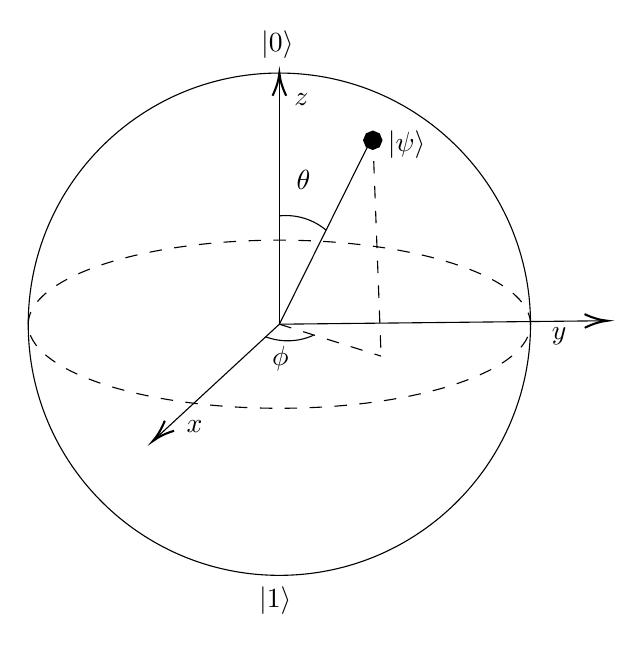
\begin{tikzpicture}[x=0.75pt,y=0.75pt,yscale=-1,xscale=1]
%uncomment if require: \path (0,300); %set diagram left start at 0, and has height of 300

%Shape: Circle [id:dp20108099716920003] 
\draw   (218,151) .. controls (218,84.17) and (272.17,30) .. (339,30) .. controls (405.83,30) and (460,84.17) .. (460,151) .. controls (460,217.83) and (405.83,272) .. (339,272) .. controls (272.17,272) and (218,217.83) .. (218,151) -- cycle ;
%Shape: Ellipse [id:dp35147631785654676] 
\draw  [dash pattern={on 4.5pt off 4.5pt}] (218,151) .. controls (218,128.63) and (272.17,110.5) .. (339,110.5) .. controls (405.83,110.5) and (460,128.63) .. (460,151) .. controls (460,173.37) and (405.83,191.5) .. (339,191.5) .. controls (272.17,191.5) and (218,173.37) .. (218,151) -- cycle ;
%Straight Lines [id:da9737644492660524] 
\draw    (339,151) -- (279.47,205.98) ;
\draw [shift={(278,207.33)}, rotate = 317.28] [color={rgb, 255:red, 0; green, 0; blue, 0 }  ][line width=0.75]    (10.93,-3.29) .. controls (6.95,-1.4) and (3.31,-0.3) .. (0,0) .. controls (3.31,0.3) and (6.95,1.4) .. (10.93,3.29)   ;
%Straight Lines [id:da9485274003962265] 
\draw    (339,151) -- (495,149.35) ;
\draw [shift={(497,149.33)}, rotate = 539.4] [color={rgb, 255:red, 0; green, 0; blue, 0 }  ][line width=0.75]    (10.93,-3.29) .. controls (6.95,-1.4) and (3.31,-0.3) .. (0,0) .. controls (3.31,0.3) and (6.95,1.4) .. (10.93,3.29)   ;
%Straight Lines [id:da34424172783269724] 
\draw    (339,151) -- (339,32) ;
\draw [shift={(339,30)}, rotate = 450] [color={rgb, 255:red, 0; green, 0; blue, 0 }  ][line width=0.75]    (10.93,-3.29) .. controls (6.95,-1.4) and (3.31,-0.3) .. (0,0) .. controls (3.31,0.3) and (6.95,1.4) .. (10.93,3.29)   ;
%Shape: Circle [id:dp48820869607163986] 
\draw  [line width=3.75]  (382.01,62.38) .. controls (382.01,61.28) and (382.9,60.39) .. (384,60.39) .. controls (385.11,60.39) and (386,61.28) .. (386,62.38) .. controls (386,63.49) and (385.11,64.38) .. (384,64.38) .. controls (382.9,64.38) and (382.01,63.49) .. (382.01,62.38) -- cycle ;
%Straight Lines [id:da06989304326514079] 
\draw    (339,151) -- (384,60.39) ;
%Straight Lines [id:da11499956861011906] 
\draw  [dash pattern={on 4.5pt off 4.5pt}]  (384,60.39) -- (388.01,166.38) ;
%Straight Lines [id:da9948469036455292] 
\draw  [dash pattern={on 4.5pt off 4.5pt}]  (339,151) -- (388.01,166.38) ;
%Shape: Arc [id:dp07709674009242451] 
\draw  [draw opacity=0] (355.43,156.31) .. controls (348.12,159.64) and (339.75,159.88) .. (332.29,157.03) -- (343,129) -- cycle ; \draw   (355.43,156.31) .. controls (348.12,159.64) and (339.75,159.88) .. (332.29,157.03) ;
%Shape: Arc [id:dp077081113703378] 
\draw  [draw opacity=0] (339.15,98.8) .. controls (347.23,97.98) and (355.32,100.5) .. (361.5,105.69) -- (342.18,128.65) -- cycle ; \draw   (339.15,98.8) .. controls (347.23,97.98) and (355.32,100.5) .. (361.5,105.69) ;

% Text Node
\draw (329,8.4) node [anchor=north west][inner sep=0.75pt]    {$|0\rangle $};
% Text Node
\draw (328,276.4) node [anchor=north west][inner sep=0.75pt]    {$|1\rangle $};
% Text Node
\draw (469,151.4) node [anchor=north west][inner sep=0.75pt]    {$y$};
% Text Node
\draw (293,196.4) node [anchor=north west][inner sep=0.75pt]    {$x$};
% Text Node
\draw (345,38.4) node [anchor=north west][inner sep=0.75pt]    {$z$};
% Text Node
\draw (334.29,160.43) node [anchor=north west][inner sep=0.75pt]    {$\phi $};
% Text Node
\draw (346,75.4) node [anchor=north west][inner sep=0.75pt]    {$\theta $};
% Text Node
\draw (390,56.4) node [anchor=north west][inner sep=0.75pt]    {$|\psi \rangle $};



    \end{tikzpicture}

    \caption{The Bloch Sphere}
    \label{fig:Blochmy}
\end{figure}

From this representation we can find the probability of $|\psi \rangle$ collapsing to $|\phi_0 \rangle$ to be $\frac{1}{2}(1+cos(\theta)$ \cite{QRAC2009}. 

For a $2 \xrightarrow[\text{}]{\text{p}} 1$ QRAC the probability threshold is just $\frac{1}{2}+\frac{1}{2\sqrt{2}}\approx 0.85$ \cite{ambainis1998dense}, and for  $3 \xrightarrow[\text{}]{\text{p}} 1$ it is $\frac{1}{2}+\frac{1}{2\sqrt{3}}\approx 0.79$ \cite{ILChaung}. Let us assume the minimum probability threshold is 0.5 (better than a coin flip). For a  $n \xrightarrow[\text{}]{\text{p}} 1$ to have a probability greater than 0.5, a sphere must be able to be divided into $2^n$ parts (as our minimum probability is 0.5) by n planes. As you can see, in the figure below, it is possible to cut a sphere into four parts using two planes and eight parts using three planes, but it is impossible to cut a sphere into 16 parts using four planes, we can at most cut it into 14 parts. Hence a $4 \xrightarrow[\text{}]{\text{p}} 1$ never works for $p>1/2$ \cite{41}.
\begin{figure}

\begin{minipage}{.5\linewidth}
\centering
\subfloat[]{\label{main:a}\includegraphics[scale=.125]{Images/QRACBloch.png}}
\end{minipage}%
\begin{minipage}{.5\linewidth}
\centering
\subfloat[]{\label{main:b}\includegraphics[scale=.125]{Images/QRACBloch 2.png}}
\end{minipage}\par\medskip
\centering
\subfloat[]{\label{main:c}\includegraphics[scale=.125]{Images/QRACBloch 3.png}}

\caption{ A sphere can be cut into a. four regions by two plane b. eight regions by two planes c. but it can be cut into at most 14 regions by 3 planes }
\label{fig:spherecutter}
\end{figure}

\subsubsection{Communication complexities:}

The main aim of finding communication complexity is to calculate the number of communication bits that Alice and Bob must exchange in order to perform a certain task. The simplest example is that proposed by Yao (\cite{Yao1979}), where Alice and Bob each have bits x and y, bits, respectively. They need to send these bits to a third party (the referee), and then all three collectively need to calculate the value of a function f(x,y) while minimizing the amount of information used. 
\begin{equation}
f(x)=
\begin{cases} 
1, & x\neq y\\
0, & x=y
\end{cases}
\end{equation}

A trivial communication strategy is just Alice sending x to the referee and Bob sending y to the referee but this is highly inefficient with a complexity of $O(2n)$ (sending two bits of length n). The "communication cost" of this strategy could be highly reduced if only a part of the bit is sent instead of the whole bit. This is where tools like Quantum fingerprinting can be applied, and used to distinguish two strings by using the least amount of bits. Instead of comparing the entire string, only the fingerprint of the string will be compared which reduces the communication complexity significantly.

Another way to decrease the communication complexity is to use the concept of shared randomness, where since Alice and Bob are entangled, less amount of information transfer is needed.



\subsection{Quantum Data Locking (QDL):}

The idea behind QDL is pretty simple, Alice and Bob initially share no mutual information, now Alice using a key of length k encodes a n-bit message into a n-bit code-word sends the code-word to Bob. They now share a mutual information of n. When Alice shares the key, the mutual information could potentially increase by more than k by quantum mechanical means. Now, the regular BB84 protocol follows but with an important difference: in QDL Eve is assumed to be able to store quantum information only for a limited time or a limited amount of information can be stored at any time. What this means is that, if Eve intercepts n qubits she has to measure them instantaneously (or after some time), she cannot gain all the information. The amount of information that Eve can extract from a quantum system is called the accessible information; in this case Eve can only have a maximum information of $\frac{n}{2}$. Thus, Eve loses half the information, and if the length of the bit is long enough the information Eve has would be negligible. In addition, for any QDL protocol to be deemed "good", the length of the message transferable should be much greater than the length of the key itself. QDL works best for locking information in quantum states using exponentially small pre-shared keys \cite{Liu_2016}.

\subsection{Quantum Digital Signatures (QDS):}

In cryptography, many a times we need to verify the origin of a message. This can be achieved by using a digital signature.

A classical digital signature is very similar to the way asymmetric cryptosystems work, by using one-way functions (Given x we find f(x) but not the other way around). A common one-way function used is prime-factoring, but as we know, no provably secure one-way function has been found. For example,the prime factoring function is not secure against a quantum computer. This leaves a hole in cryptography which quantum signatures attempts to fill.

A QDS Scheme ensures that:
\begin{enumerate}
    \item The message was created by the sender, which he cannot deny
    \item The message has not been tampered with
    \item The message if accepted at one receiver should be acceptable at all receivers
\end{enumerate}

\subsubsection{The Gottesman-Chuang protocol:}

The Gottesman-Chaung protocol uses the ideas of  quantum one-way function, similar to classical one way functions, they return a public quantum bit-key from a provate classical/quantum string \cite{gottesman2001quantum}.



In a simplified Gottesman scheme we consider the former case of using a classical string. It goes as follows:

As we can see, Alice has to sign every bit in the message. For this she chooses R pairs of private keys ${k^j_0, k^j_1} \ \ (0\ <\ j\ <\ R$, where all $k^j_0$ will be used to sign bit 0 and all $k^j_1$ will be used to sign bit 1. The function ${\displaystyle k\mapsto |f_{k}\rangle }k\mapsto |f_{k}\rangle$ is public and Alice converts $k^j_0$ and $k^j_1$ into $|f^j_{k_0}\rangle$ and $|f^j_{k_1\rangle}$, the public quantum keys. She can make as many identical copies of these keys as she wants but more the number of copies lesser the security of the system. ,Now she sends this to Bob, who now has the bit a, private keys, and their corresponding public keys. Bob now uses the $k_a$ and calculates the value of $|f_{k_a}\rangle$.  

But a problem arises here, lets say we have two quantum states $|f_k\rangle$ and $|f'_k\rangle$, how do we find out if they are the same? Classically this problem is trivial, as we can just look at the strings and find out if they are the same. However, it becomes interesting when we look at it quantum mechanically. We perform the SWAP test to achieve this, instead of delving into the details, all we need to know about the SWAP test is that it is not deterministic. There is always a probability that it gives you the wrong answer. 

What this means is that Bob can compare the values of $f^j_{k_a}$ that he found with ${f^j_{k_0}, f^j_{k_0}}$ and as we discussed earlier the SWAP test can give incoorect results, therefore there will be a few mismatched bits (m). Now, as long as m is below a certain pre-fixed threshold Bob accepts the signature or else He rejects them as forgeries.



\section{Conclusions}

Quantum Cryptography is a beautiful combination of information theory and the laws of quantum mechanics. In our review we presented the basic laws of quantum mechanics, delved into a few Key distribution protocols, looked and how to counter eavesdroppers, real life attacks and finally at some non-key distribution protocols like data locking and digital signatures. The tremendous progress in quantum optics and optical fibers makes such protocols to be realised in the real world. Privacy Amplification (Sec X.), is a classical protocol heavily inspired from Quantum Cryptography. Though, Quantum Cryptography is mature there are still a lot of technological challenges that remain.

For example, the compatibility of the advanced detectors with the communication fibers. Another issue of Quantum Cryptography concerns its range, QC protocols even with modern range technology have a short distance range compared to other communication methods. Practical quantum repeaters could be the key for long range QC. Quantum repeaters detect and correct errors, provided error rate is low enough. We can hope that such techniques could potentially lead to realise QC over long distances. QC's however still have many loopholes like side channel attacks, errors in random number generators and imperfection in the detectors which Eavesdropper's can Exploit. 

Despite these loopholes, humanity will master this technology and QC will become a commercial product potentially for secure financial transactions among other applications, we just do not know when that is going to happen.



%\appendix
%here
\bibliography{biblio.bib}
\end{document}
